%======================================================================
\chapter{Background}
%======================================================================
\section{Hollow-Core Photonic Crystal Fiber}
\subsection{Conventional TIR Guidance}

\subsection{Photonic Crystal Bandgap}

The 1D and 2D views of the structure
\begin{figure}
	\centering
	\begin{tabular}{cc}
		\multirow{-3}[15]{*}{\subfloat[]{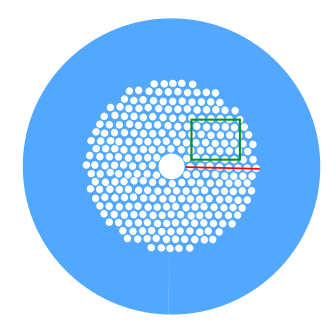
\includegraphics[width=7cm,height=7cm]{./Figures/HCPCF/HCPCF_section.png}}} &
		\subfloat[]{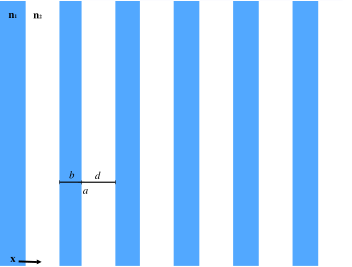
\includegraphics[width=4.5cm,height=3.5cm]{./Figures/HCPCF/HCPCF_1D.png}}                          \\&
		\subfloat[]{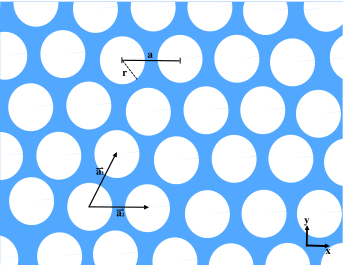
\includegraphics[width=4.5cm,height=3.5cm]{./Figures/HCPCF/HCPCF2D.png}}
	\end{tabular}
	\hfill
	\caption{(a)cross-section of HCPCF highlighting the PC pattern (b)reduced to 1-dimension (2)in 2-dimensions}
	\label{fig:manyD}
\end{figure}

A periodic non-magnetic medium will have repeating dielectric constant \cite{yariv}
\begin{equation}
	\varepsilon(\boldsymbol{r}) = \varepsilon(\boldsymbol{r}+\boldsymbol{a})
\end{equation}
Due to its discrete and invariant translational symmetry, the dielectric constant along the medium can be expanded as the Fourier series
\begin{equation}
	\varepsilon(\boldsymbol{r}) = \sum_{\boldsymbol{G}}\varepsilon_{\boldsymbol{G}}e^{i\boldsymbol{G}\cdot\boldsymbol{r}}
	\label{eqn:fourier_eps}
\end{equation}
where $\boldsymbol{G}$ are the reciprocal lattice vectors such that $\boldsymbol{G}\cdot\boldsymbol{a} = 2\pi n$. We can express the electric field also as the Fourier integral
\begin{equation}
	\boldsymbol{E}(\boldsymbol{r}) = \iiint d^3\boldsymbol{k}\boldsymbol{A}(\boldsymbol{k})e^{i\boldsymbol{k}\cdot\boldsymbol{r}}
	\label{eqn:fourier_E}
\end{equation}
Using the Maxwell equations (\ref{eqn:maxwell}) the wave equation can be written in terms of the electric field
\begin{equation}
	\begin{aligned}
		\begin{cases}
			\vec{\nabla}\times\vec{H} & = -i\omega\epsilon(\vec{r})\vec{E} \\
			\vec{\nabla}\times\vec{E} & = i\omega\mu_0\vec{H}
		\end{cases}
	\end{aligned}
	\label{eqn:maxwell}
\end{equation}
\begin{equation}
	\boldsymbol{\nabla}\times(\boldsymbol{\nabla}\times\boldsymbol{E})-\omega^2\varepsilon(\boldsymbol{r})\mu_0\boldsymbol{E} = 0
\end{equation}
Substituting \eqref{eqn:fourier_eps} and \eqref{eqn:fourier_E} into the above results in the dispersion relation:
\begin{equation}
	\boldsymbol{k}\times(\boldsymbol{k}\times\boldsymbol{A}(\boldsymbol{k})) + \omega^2\mu_0\sum_{\boldsymbol{G}}\varepsilon_{\boldsymbol{G}}\boldsymbol{A}(\boldsymbol{k}-\boldsymbol{G}) = 0
	\label{eqn:separation}
\end{equation}
in where for any vector $\boldsymbol{K}$ the solutions of \eqref{eqn:separation} for the coefficient $\boldsymbol{A}(\boldsymbol{K})$ are grouped with the coefficients $\boldsymbol{A}(\boldsymbol{K}-\boldsymbol{G})$, decoupling the coefficients of other vectors that cannot be expressed in the form $\boldsymbol{K}-\boldsymbol{G}$. Disregarding the decoupled vectors, the total electric field can be described as a superposition of normal modes with regard to a chosen vector $\boldsymbol{K}$ :
\begin{equation}
	\boldsymbol{E}_{\boldsymbol{k}}(\boldsymbol{r}) = \sum_{\boldsymbol{G}}\boldsymbol{A}(\boldsymbol{K}-\boldsymbol{G})e^{i(\boldsymbol{k}-\boldsymbol{G})\cdot \boldsymbol{r}}
	\label{eqn:normalmodes}
\end{equation}
we can pull out the Bloch theorem for the electric field from \eqref{eqn:normalmodes}
\begin{equation}
	\boldsymbol{E}_{\boldsymbol{k}}(\boldsymbol{r}+\boldsymbol{a}) = e^{i\boldsymbol{k}\cdot \boldsymbol{a}}\boldsymbol{E}_{\boldsymbol{k}}(\boldsymbol{r})
\end{equation}
\begin{equation}
	\boldsymbol{u_k}(\boldsymbol{r}) = \sum_{\boldsymbol{G}}\varepsilon_{\boldsymbol{G}}e^{i\boldsymbol{G}\cdot\boldsymbol{r}}
\end{equation}
\begin{equation}
	\varepsilon_{\boldsymbol{G}} = \frac{1}{V}\int d^3\boldsymbol{r}e^{-i\boldsymbol{G}\cdot\boldsymbol{r}}\boldsymbol{u_k}(\boldsymbol{r})
	\label{eqn:perm}
\end{equation}
(Expand)  Returning to \eqref{eqn:separation}, can fix $\omega$ to find the corresponding $\boldsymbol{K}$ and normal modes os the system. However, in the case of photonic crystals there are ranges of frequencies that  have no $\boldsymbol{K}$s with real solutions, which implies that waves of these frequencies cannot propagate through the photonic crystal. These non-propagating frequencies are referred to as the photonic band gap.

\subsubsection{1D Photonic Bandgap}
Returning to the 1D periodic stack pictured in Fig. \ref{fig:manyD} the periodicity of dielectric constant is described by $\varepsilon(z) = \varepsilon(z+p)$ where $a = b+d$, the length of one period. The reciprocal lattice vector will be $\boldsymbol{G}_n = n\frac{2\pi}{a}\hat{z}$ and plugging into the Fourier series expansion of $\varepsilon(z)$  from \eqref{eqn:fourier_eps}
\begin{equation}
	\varepsilon(z)  =\sum_{n=-\infty}^\infty\varepsilon_ne^{in\frac{2\pi}{a}\hat{z}}
\end{equation}
From the reduction to propagation in the z-direction with the electric field oriented in x-direction, \eqref{eqn:separation} simplifies
\begin{equation}
	K^2A(K) + \omega^2\mu_0\sum_{n=-i\infty}^\infty\varepsilon_nA(K-n\frac{2\pi}{a}) = 0
\end{equation}
Expanding the Fourier coefficients to the 1st order and reducing the equations to the dominant coefficients of the form $A(K)$ and $A(K-\frac{2\pi}{a})$ . $|K - g| = K$ and $K = \frac{\pi}{a}$ gives a system of equations that can be solved to find the dispersion relation $\omega(K)$.
\begin{equation}
	\begin{cases}
		\big(K^2-\omega^2\mu_0\varepsilon_{00}\big)A(K) = \omega^2\mu_0\varepsilon_1A(K - g) \\
		\omega^2\mu_0\varepsilon_{-1}A(K) = \big((K-g)^2-\omega^2\mu_0\varepsilon_{00}\big)A(K-g)
	\end{cases}
\end{equation}
The equations relating these two modes has a solution at
\begin{equation}
	\big(K^2-\omega^2\mu_0\varepsilon_{00}\big)\big((K-g)^2-\omega^2\mu_0\varepsilon_{00}\big) -\big(\omega^2\mu_0\varepsilon_1\big)\big(\omega^2\mu_0\varepsilon_{-1}\big)  = 0
\end{equation}
noting $\varepsilon_1 = \varepsilon_{-1}^*$ and $K\approx2g$ simplifies the relationship
\begin{equation}
	\omega_{\pm}^2 = \frac{K^2}{\mu_0(\varepsilon_{00}\mp|\varepsilon_1|)}
\end{equation}
The dispersion relation has two possible solutions, which specify the top and bottom of the photonic bandgap edges, as illustrated in Fig. \ref{fig:1dbp}.
\begin{figure}[h]
	\centering
	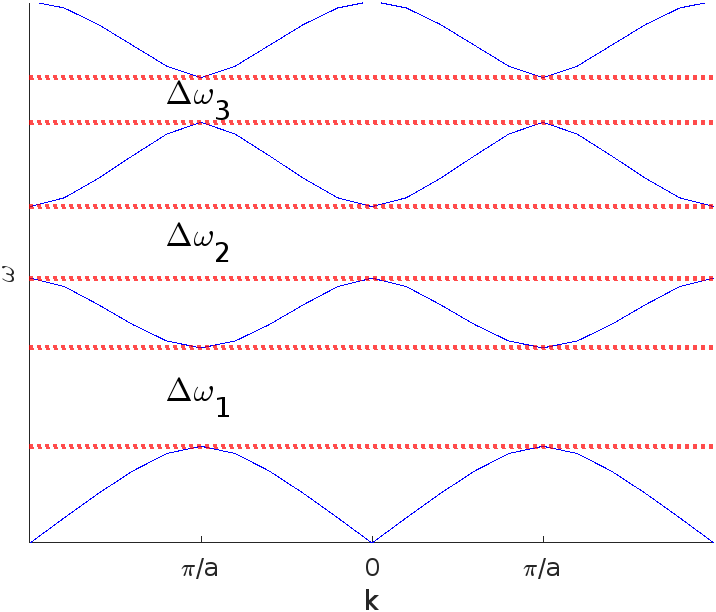
\includegraphics[width=0.6\textwidth]{./Figures/HCPCF/1D_BandGap.png}
	\caption {Band plot for a 1D photonic crystal with parameters-,-, solved using Finite Difference Time Domain(FDTD) method\cite{sukhoivanov}.}
	\label{fig:1dbp}
\end{figure}

If solving for the wavevector at a frequency between the two roots $\omega_{\pm}$, only complex solutions will exist. This means that only evanescent waves, not electromagnetic waves, propagate through the medium while the electromagnetic waves are reflected back; the medium acts as a mirror for the bandgap wavelengths.\\
This is the the phenomenon that allows for HCPCF to guide certain frequencies of light: wavelengths in the bandgap are reflected by surrounding Bragg Grating confining them to the core of the fiber, while the rest are allowed to propagate through the grating.

\subsubsection{2D Photonic Bandgap}
To understand the full picture of light propagation in hollow-core fiber, we need to expand to the 2D case pictured in Fig. \ref{fig:manyD}c. However, with the electromagnetic waves now propagating in two dimension there is an added layer of complexity with the TE TM wave polarizations and the bandgaps. In addition to controlling the refractive index of the material and the period of the lattice, the lattice structure and hole radius will affect the performance of the photonic crystal, the latter playing a large role in the completeness of the photonic bandgap. In the 2D photonic crystal, the in-plane guided modes will have either magnetic fields in-plane and electric fields perpendicular to the lattice (TE modes), or electric fields in-plane and magnetic fields perpendicular to the lattice (TM modes). As the TE and TM modes are perpendicular to each other they may exhibit wildly different dispersion relations, which means that an optical bandgap is not guaranteed to persist for all polarizations\cite{joannopoulos}. This is certainly the case for square lattice phonic crystals, but  other patterns such as the honeycomb (which is the structure in our HCPCF) do have a bandgap persisting for all polarizations\cite{villeneuve}. This all to say, it is important to consider all polarization effects when making decisions about photonic crystal patterns for two or more dimensions. \\
\begin{figure}[h]
	\centering
	\foreach \x in {HCPCF_2D_cartesian, HCPCF_2D_reciprocal}
		{
			\begin{subfigure}[b]{0.45\textwidth}
				\includegraphics[width=\textwidth]{./Figures/HCPCF/\x.png}
				\caption{}
			\end{subfigure}
			\hfil
		}
	\caption {(a) primitive lattice vectors and (b) primitive reciprocal lattice vectors with first Brillouin zone (green) and irreducible  Brillouin  zone (red) depicted for a honeycomb lattice structure.  }
	\label{fig:2d}
\end{figure}
\clearpage
Considering the lattice structure in Fig. \ref{fig:2d}(a), and taking propagation in the xy-plane ($K_z=0$ and $z=0$ for simplicity), the wavevector and position vectors reduce to  $\boldsymbol{K_{||}}=k_x\hat{x}+k_y\hat{y}$ and $\boldsymbol{r_{||}}=x\hat{x}+y\hat{y}$.  The primitive lattice vectors of a honeycomb photonic crystal will be:
\begin{equation}
	\boldsymbol{a}_1 = a\hat{x} \hspace{1cm} \boldsymbol{a}_2 = \frac{a}{2}\hat{x}+\frac{a\sqrt{3}}{2}\hat{y}
\end{equation}
and transforming to the momentum-space,  $\boldsymbol{b}\cdot\boldsymbol{a} = 2\pi\delta_{ij}$, as shown in Fig. \ref{fig:2d}(b) the primitive reciprocal lattice vectors are
\begin{equation}
	\boldsymbol{b}_1 = \frac{2\pi}{a}\hat{x}-\frac{2\pi}{a\sqrt{3}}\hat{y} \hspace{1cm} \boldsymbol{b}_2 =\frac{4\pi}{a\sqrt{3}}\hat{y}
\end{equation}
Taking these in combination of $n, m$ integer scaling factors, the reciprocal lattice vector is defined $\boldsymbol{G_{||}} = n\boldsymbol{b}_1 + m\boldsymbol{b}_2$.
The electromagnetic field defined for a two dimensional system
\begin{equation}
	\boldsymbol{E}(\boldsymbol{r}) = e^{i\boldsymbol{k}\cdot\boldsymbol{r}}
	\sum_{m=-\infty}^\infty\sum_{n=-\infty}^\infty\boldsymbol{E}_{m,n}
	e^{i(n\boldsymbol{b_1}+m\boldsymbol{b_2})\cdot\boldsymbol{r}}
	\label{eqn:2d_emf}
\end{equation}
and the correlating Fourier expansion of dielectric function \eqref{eqn:perm}
\begin{equation}
	\varepsilon_{\boldsymbol{G_{||}}} = \frac{1}{a'\cdot b'}\int dxdye^{i(G_xx + G_yy)}\boldsymbol{u_k}(x, y)
	\label{eqn:2d_perm}
\end{equation}
are substituted into \eqref{eqn:maxwell}.
Utilizing the lattice symmetry and periodicity, the problem can be restricted to only solve for Bloch modes inside the of the irreducible Brillouin zone.
The first Brillouin zone is defined by the perpendicular bisectors to the primitive reciprocal lattice vectors, depicted in green in Fig. \ref{fig:2d}(b) and can be further subdivided into the irreducible Brillouin zone shown in red.
In order to find the photonic bandgap, solving the dispersion equation just along the irreducible Brillouin zone is sufficient.
For a honeycomb lattice, the $k$-path to follow would be
\begin{equation}
	\begin{cases}
		|\Gamma X| = \frac{2\pi}{a\sqrt{3}}, & k_x=0, 0<k_y<\frac{2\pi}{\sqrt{3}a}               \\
		|XJ| =  \frac{2\pi}{3a},             & 0<k_x<\frac{2\pi}{3a}, k_y=\frac{2\pi}{\sqrt{3}a} \\
		|\Gamma J| = \frac{4\pi}{3a},        & 0<k_x<\frac{2\pi}{3a}, k_y=\sqrt{3}k_x
	\end{cases}
\end{equation}
Discretizing  (\ref{eqn:2d_emf}) and (\ref{eqn:2d_perm}) then picking a few points along the $k$-path, numerical methods can be used to solve for the optical bandgap. Fig. \ref{fig:2dbp} shows the resulting TE bandgap for a honeycomb lattice with parameters-,-, using Plane Wave Expansion(PWE)\cite{sukhoivanov}.
\begin{figure}[h]
	\centering
	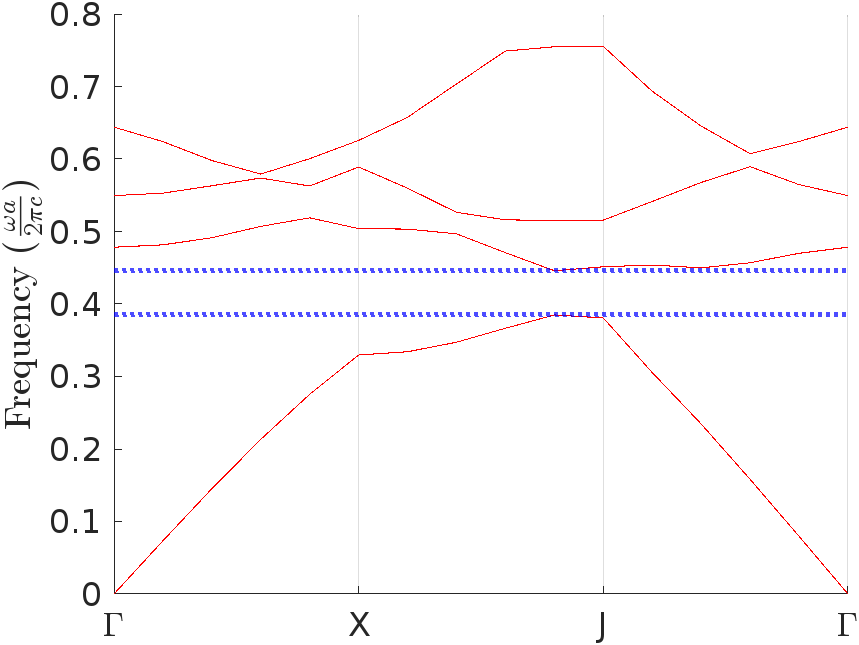
\includegraphics[width=0.8\textwidth]{./Figures/HCPCF/2D_BandDiagram.png}
	\caption {Band plot along the irreducible Brillouin zone for a honeycomb lattice with parameters -,-, . Solved for using Plane Wave Expansion(PWE) numerical method\cite{sukhoivanov}.}
	\label{fig:2dbp}
\end{figure}

\clearpage
\subsection{Bandgap Shift}
The modal magnetic field distributions satisfy:
\begin{equation}
	(\nabla^2_t + k^2n(\boldsymbol{r})^2 - \beta)\boldsymbol{H(r)} = (\nabla_t\times\boldsymbol{H(r)})\times(\nabla_t ln(n(\boldsymbol{r})^2))
\end{equation}
This equation gives a scaling law for absolute refractive index at fixed contrast:
``a solution for a transverse scale represented by $\Lambda$is replicated in an identical structure with a different $\Lambda$ if the wavelength is scaled proportionately, to keep $k\Lambda$ constant''\\
``We emphasise that the scalar wave equation (and therefore the scaling laws derived from it) is accurate for the smallest index contrasts only. However, for step-index structures the vector term in Eq. (2) only exists at boundaries, so the scalar wave equation accurately represents wave propagation elsewhere. Since bandgaps arise from interference and resonance effects among such generic waves, the scaling laws of Eq. (5) should be at least approximately valid'' ~1.45 RI contrast\cite{birks}

Scaling law for the wave equation for the transverse coordinates
$X=x\Lambda^{-1}$ $Y=y\Lambda^{-1}$
where $\Lambda$ is a solution to the transverse scale.
\begin{equation}
	n(X, Y) = \begin{cases}
		1, & n_1 \text{   (high RI)} \\
		0, & n_2 \text{   (low RI)}
	\end{cases}
\end{equation}
normalized scaled wave equation:
\begin{equation}
	\nabla_\perp^2\Psi + (v^2n(X, Y) - w^2)\Psi = 0
\end{equation}
With $\nabla_\perp = \partial^2/\partial X^2 + \partial^2/\partial Y^2 $
solving for the frequency parameter $v^2$ and eigenvalue $w^2$:
\begin{equation}
	\begin{aligned}
		v^2 & = \Lambda^2k^2(n_1^2 - n_2^2)   \\
		w^2 & = \Lambda^2(\beta^2 - k^2n_2^2)
	\end{aligned}
\end{equation}
from the equation above we see that the $w^2$ is determined by the frequency parameter $v^2$ and the index distribution function $n(X, Y)$.
This implies that $w^2$ and $v^2$ are invariant with changes to the parameters $k, \Lambda, n_1, n_2$.
$k = \omega/c$ $\beta = kcos\theta$ longitudinal component of the wavevector. Because the light propagates along the fiber, much of its wavevector is taken up by the longitudinal component.

In the HCPCF case where the glass refractive index is held constant and the air in the fiber is replaced by a new material the equations can be rewritten with $n_1 = n_{glass}$ and $n_2 = n_{air}=1$:
\begin{equation}
	\begin{aligned}
		v^2 - w^2 & = \Lambda^2(k^2n_{glass} - \beta^2)                          \\
		v         & = k\Lambda n_{glass}\sqrt{n_{air} - \frac{n_{air}}{n_{new}}}
	\end{aligned}
\end{equation}
The initial index contrast $N_0 = \frac{n_{air}}{n_{glass}}$ moves to$ N = \frac{n_{new}}{n_{glass}}$ with the change in RI $n_{air} <  n_{new} < n_{glass}$
This leads to the new center bandgap to be governed by the equation:
\begin{equation}
	\lambda = \lambda_0\sqrt{\frac{1-N^{-2}}{1-N_0^{-2}}}
\end{equation}
This has been experimentally confirmed to hold for HCPCF \cite{antonopoulos}.




